\documentclass[10pt,aspectratio=169]{ctexbeamer}
\usetheme{Madrid}
\usecolortheme{default}
\usepackage{graphicx}

% === 基本信息 ===
\title{腐蚀领域学术摘要文体特征与影响力关联分析}
\subtitle{扩大化基线测试结果汇报}
\author{石洪旭}
\date{\today}
\institute{上海理工大学}

\begin{document}

% ============================================
\begin{frame}
\titlepage
\end{frame}

% ============================================
\section{研究背景}

\begin{frame}{研究背景}
  \begin{block}{核心问题}
    学术摘要的文体特征是否与论文影响力（被引次数）存在关联？
  \end{block}

  \begin{itemize}
    \item \textbf{研究对象}：腐蚀科学领域英文论文摘要
    \item \textbf{基线阶段}：Corrosion Science 期刊 2023 年论文，共 377 篇
    \item \textbf{扩大阶段}：6 本腐蚀期刊 2015--2026 年论文，共 5{,}821 篇
    \item \textbf{影响力指标}：规范化引用计数 NCC（期刊$\times$年份双维度归一化）
  \end{itemize}
\end{frame}

% ============================================
\section{数据规模}

\begin{frame}{数据规模对比}
  \begin{columns}[T]
    \begin{column}{0.45\textwidth}
      \centering
      \begin{tabular}{lcc}
        \hline
        & 基线 & 扩大 \\
        \hline
        样本量     & 377      & \textbf{5{,}821} \\
        期刊数     & 1        & \textbf{6} \\
        年份范围   & 2023     & \textbf{2015--2026} \\
        NCC 归一化 & 年份     & \textbf{期刊$\times$年份} \\
        \hline
      \end{tabular}
    \end{column}
    \begin{column}{0.55\textwidth}
      \footnotesize
      \centering
      \begin{tabular}{lr}
        \hline
        期刊 & 篇数 \\
        \hline
        Materials and Corrosion          & 1{,}820 \\
        Corrosion                        & 1{,}271 \\
        Anti-Corrosion Methods           & 895 \\
        Corrosion Engineering            & 873 \\
        Corrosion Science                & 690 \\
        Corrosion and Materials Degrad.  & 272 \\
        \hline
        \textbf{合计}                    & \textbf{5{,}821} \\
        \hline
      \end{tabular}
    \end{column}
  \end{columns}
\end{frame}

% ============================================
\section{当前特征体系}

\begin{frame}{当前特征体系（六项浅层文体特征）}
  \footnotesize
  \begin{table}
    \centering
    \begin{tabular}{cll}
      \hline
      缩写 & 特征 & 计算方式 \\
      \hline
      ASL & 平均句长       & 总词数 / 句号数 \\
      MWL & 平均词长       & 去标点字符数 / 总词数 \\
      LD  & 词汇密度       & (总词数$-$停用词) / 总词数 \\
      LC  & 词汇高级度(TTR)& 不重复词类型数 / 总词令牌数 \\
      JD  & 术语密度       & 腐蚀术语命中数 / 总词数 \\
      HD  & 模糊语密度     & 模糊限制语命中数 / 总词数 \\
      \hline
    \end{tabular}
  \end{table}

  \vspace{0.3em}
  \begin{alertblock}{已知问题}
    全部停留在词级和句级的简单计数，缺乏句法、篇章、语用维度。
  \end{alertblock}
\end{frame}

% ============================================
\section{测试一：Pearson 相关}

\begin{frame}{测试一：Pearson 相关分析}
  \begin{columns}[T]
    \begin{column}{0.4\textwidth}
      \centering
      \begin{tabular}{lcc}
        \hline
        特征 & r & 结论 \\
        \hline
        MWL & +0.07 & 可忽略 \\
        LC  & $-$0.03 & 可忽略 \\
        LD  & $-$0.02 & 可忽略 \\
        ASL & +0.01 & 可忽略 \\
        JD  & $-$0.01 & 可忽略 \\
        HD  & +0.01 & 可忽略 \\
        \hline
      \end{tabular}

      \vspace{0.8em}
      \begin{block}{结论}
        \small
        六项特征与 NCC 全部趋近于零。\\
        5{,}821 条数据确认：\textbf{线性关系不存在}。
      \end{block}
    \end{column}
    \begin{column}{0.6\textwidth}
      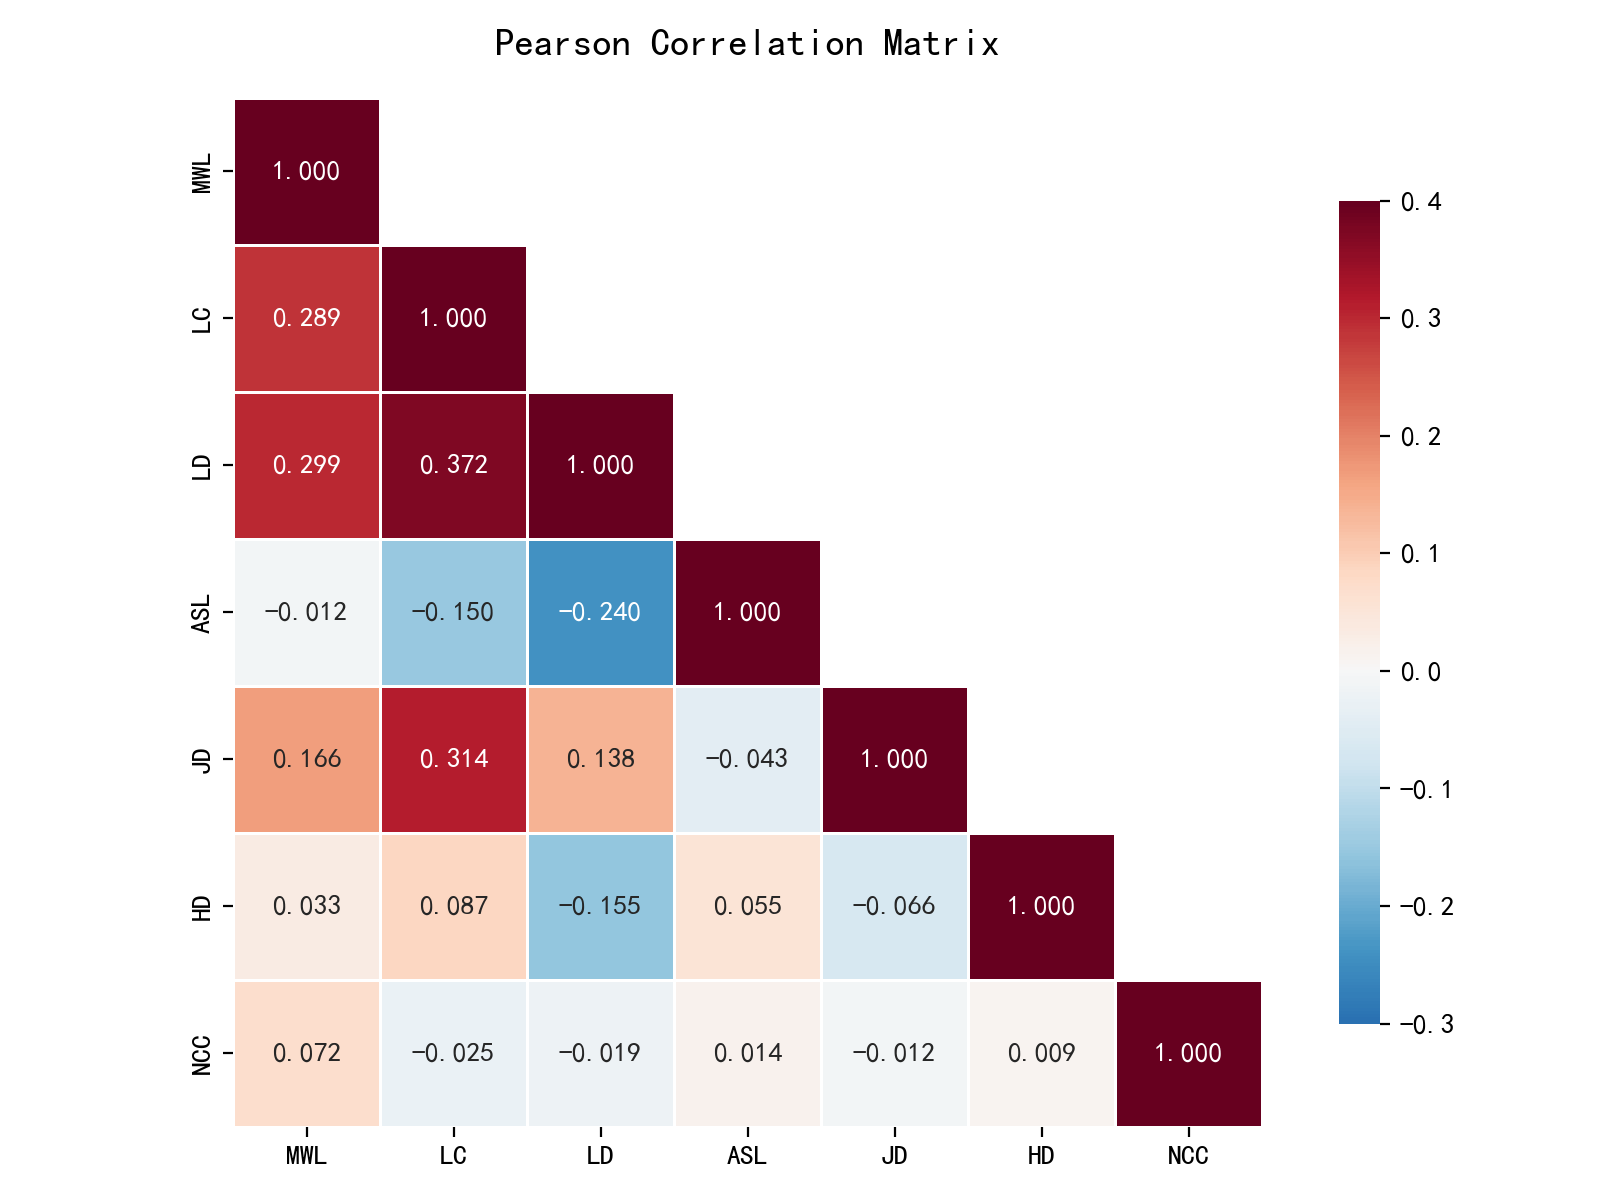
\includegraphics[width=\textwidth]{fig_correlation.png}
    \end{column}
  \end{columns}
\end{frame}

% ============================================
\section{测试二：K-Means 聚类}

\begin{frame}{测试二：K-Means 聚类分析}
  \begin{columns}[T]
    \begin{column}{0.48\textwidth}
      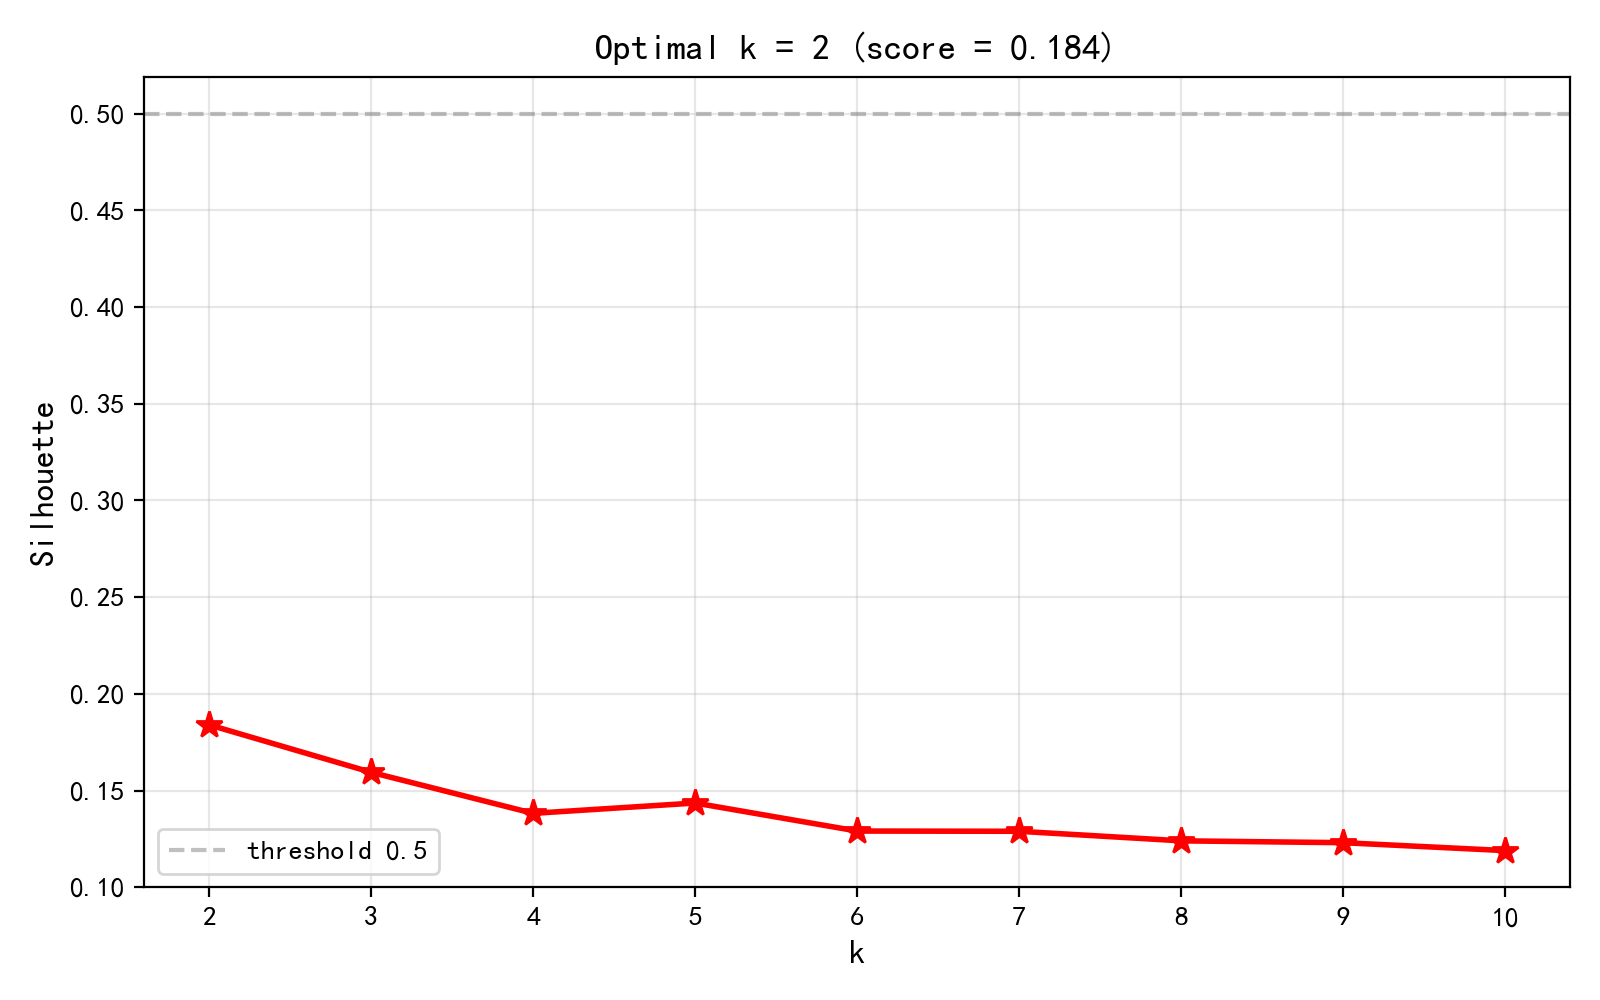
\includegraphics[width=\textwidth]{fig_silhouette.png}
    \end{column}
    \begin{column}{0.52\textwidth}
      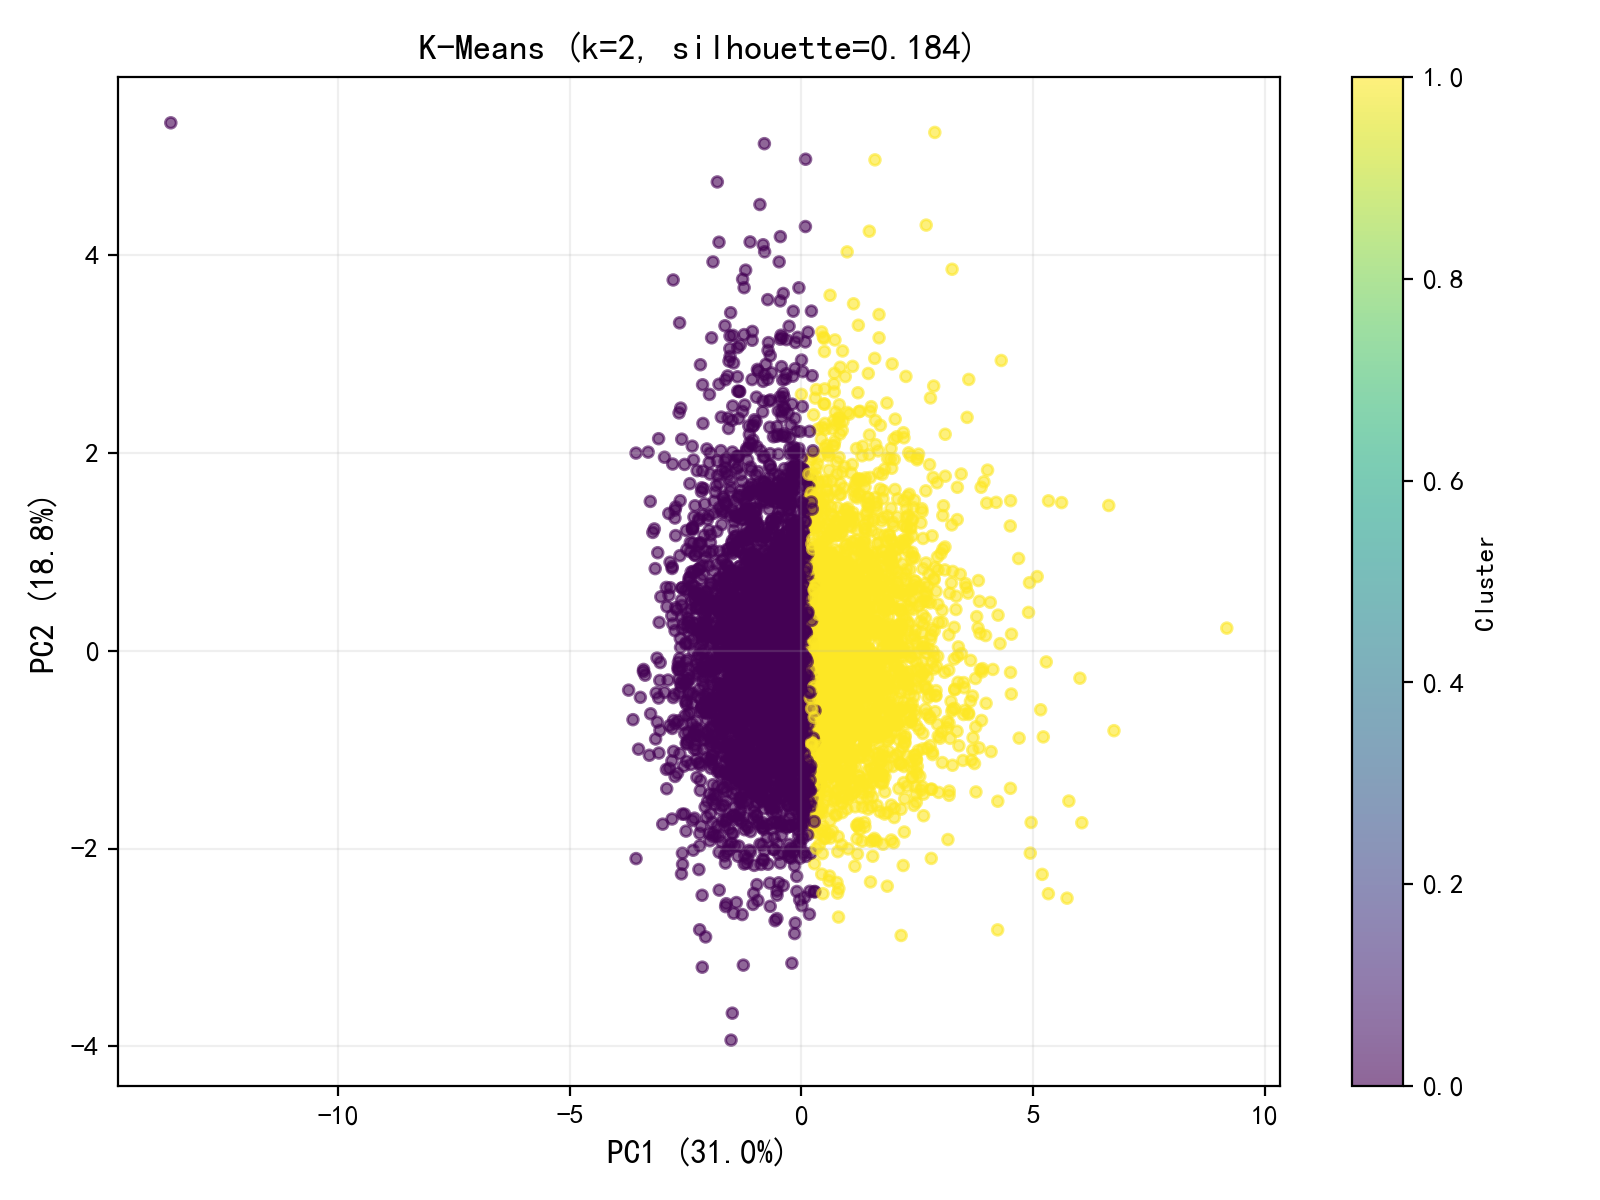
\includegraphics[width=\textwidth]{fig_pca.png}
    \end{column}
  \end{columns}
  \vspace{0.3em}
  \begin{alertblock}{结论}
    最优 $k=2$，轮廓系数仅 0.18（远低于阈值 0.5）。六项特征无法划分有意义的风格群组。
  \end{alertblock}
\end{frame}

% ============================================
\section{测试三：决策树}

\begin{frame}{测试三：决策树分类}
  \begin{columns}[T]
    \begin{column}{0.55\textwidth}
      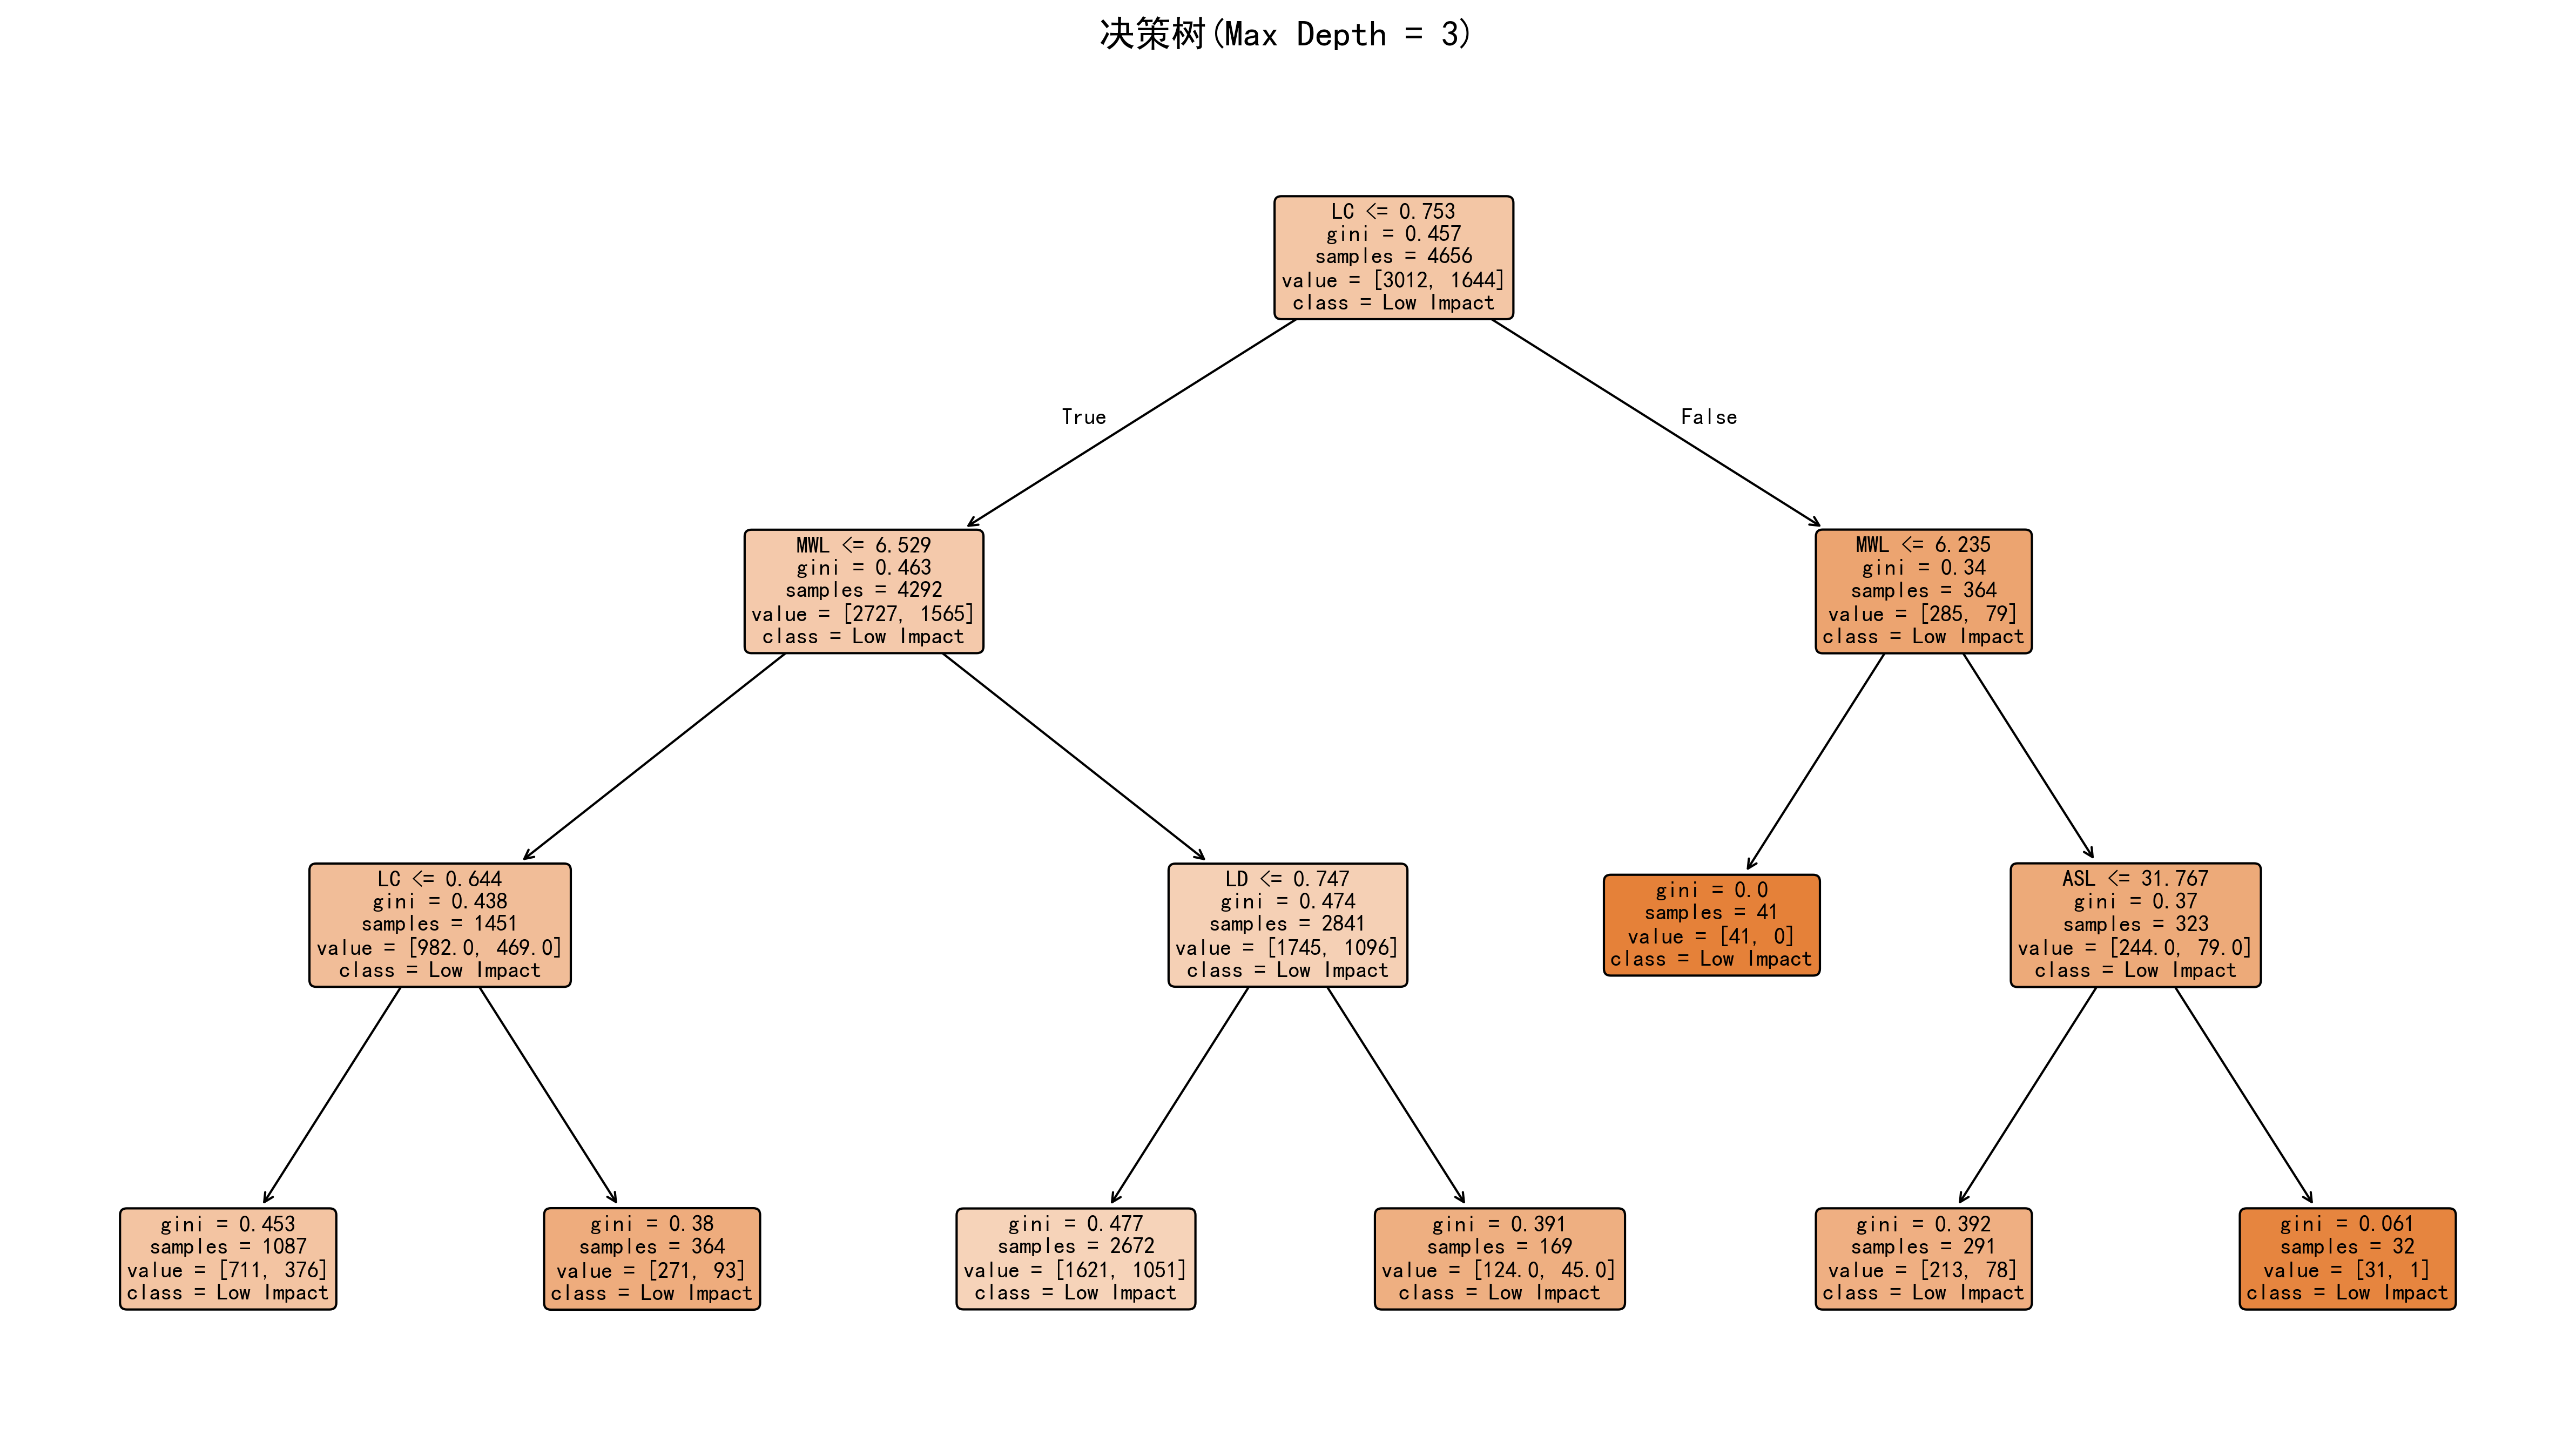
\includegraphics[width=\textwidth]{decision_tree.png}
    \end{column}
    \begin{column}{0.45\textwidth}
      \begin{block}{方法}
        \footnotesize
        NCC $\ge$ 1.0 为高影响力；max\_depth = 3 分类树
      \end{block}
      \vspace{-0.5em}
      \begin{table}
        \centering
        \begin{tabular}{lcc}
          \hline
          & 基线 & 扩大 \\
          \hline
          首要特征 & JD & \textbf{LC} \\
          准确率   & -- & \textbf{64\%} \\
          \hline
        \end{tabular}
      \end{table}
      \vspace{-0.5em}
      \begin{block}{结论}
        \small
        Accuracy $\approx$ 全猜低影响力。\\
        LC 与 JD 均为弱信号（$r=0.31$）。
      \end{block}
    \end{column}
  \end{columns}
\end{frame}

% ============================================
\section{总体结论}

\begin{frame}{总体结论}
  \begin{center}
    \Large \textbf{六项浅层文体特征对学术影响力\\没有解释或预测能力}
  \end{center}

  \vspace{0.8em}
  \begin{itemize}
    \item 相关性分析：全部趋近于零
    \item 聚类分析：无法形成有意义的风格群组
    \item 决策树分类：准确率等于随机猜测
  \end{itemize}

  \vspace{0.8em}
  \begin{block}{关键意义}
    不是"样本太小导致不显著"，而是"5{,}821 条数据上确实不成立"。
    三种方法互相印证，构成特征体系升级的实证基础。
  \end{block}
\end{frame}

% ============================================
\begin{frame}{}
  \centering
  \Large 恳请批评指正！
\end{frame}

\end{document}
